\documentclass[border = 1cm, preview, varwidth=\maxdimen]{standalone}

\usepackage{xeCJK}

% mathematics
\usepackage{amsmath}

% tikz
\usepackage{tikz}
\usepackage{ifthen}
\usetikzlibrary{arrows}
\usetikzlibrary{automata}
\usetikzlibrary{positioning}
\tikzset{->, > = stealth'}

\begin{document}
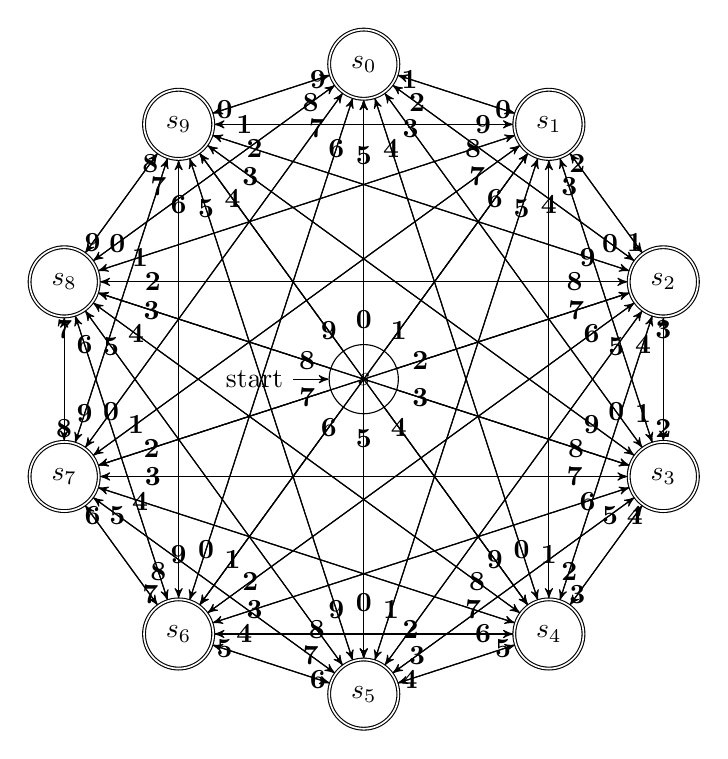
\begin{tikzpicture}
  \pgfmathtruncatemacro \digits { 10 };
  \pgfmathsetmacro \angle { 360 / \digits };
  \pgfmathtruncatemacro \n { \digits - 1 };
  % nodes
  \foreach \k in {0, ..., \n} {
    \pgfmathsetmacro \radius { 90 - \k * \angle };
    \node [state, accepting] (s\k) at (\radius:4) {$s_\k$};
  }
  \node [state, initial] (s) {$s$};
  % paths
  \foreach \i in {0, ..., \n} {
    \draw (s) edge [pos = 0.1] node {\bf\i} (s\i);
    \foreach \j in {0, ..., \n} {
      \ifthenelse {\i = \j}
        {}
        {\draw (s\i) edge [pos = 0.1] node {\bf\j} (s\j);}
    }
  }
\end{tikzpicture}
\end{document}
